\section{Introduction}
\label{sec:intro}

A customer reports a burglary. Among the stolen items is a watch that the
policy schedules separately at CHF~4,000. Under the applicable
household-insurance wording, that single fact activates an obligation that
did not exist a sentence earlier: the value of a scheduled valuable must be
established, by a purchase receipt or by an expert valuation. Remove the fact
and the obligation disappears. Leave it uncertain and the justified move is a
question, not a document request. A predictor that maps case text to a list
of documents cannot represent this dependency. It can learn that theft claims
come with receipts, and it will ask for one whether or not the case justifies
it.

\casepath is an agentic architecture in which the authoritative source, not
the language model, controls evidence acquisition. Its planning object is
the chain
\begin{equation}
\text{source}\to\text{process node}\to\text{obligation}\to
\text{required fact}\to\text{evidence capability}\to\text{document route},
\label{eq:spine}
\end{equation}
and a case's position on it is a three-valued state: every source condition
is true, false or unresolved for the case at hand. Only an active obligation
can require a fact, only a required fact can demand evidence, and only a
mapped route can name a document. Unresolved conditions produce clarification
questions rather than branch-specific requests (Figure~\ref{fig:principle}).
When new evidence is admitted, the state is recomputed and the checklist and
next action change with it. The model's roles are semantic (read a passage,
decide a condition, judge a document); code owns the consequences, so every
request carries the rule, condition and evidentiary purpose that produced it.

\begin{figure}[t]
\centering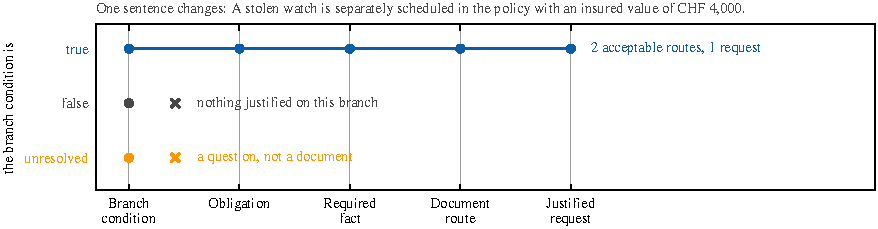
\includegraphics[width=.55\linewidth]{fig_process_principle.pdf}
\caption{\textbf{The active branch controls the request.} A source condition
makes its obligation active, inactive or unresolved. Only an active obligation
reaches a required fact, an evidence capability and a document route;
an unresolved condition yields a clarification question, never the documents
of a branch the case may not be on. New evidence updates the state and the
plan is recomputed. Acquisition permission and route sufficiency are
specified in Section~\ref{sec:method}.}
\label{fig:principle}
\end{figure}

Three questions are usually collapsed into one checklist score, and they
should not be. \emph{Traceability} asks whether a request has an inspectable
chain back to a source. \emph{Branch sensitivity} asks whether changing one
case fact changes exactly the documents that fact justifies.
\emph{Complete-case utility} asks whether a full plan covers what a case needs
without unnecessary demands. None implies the others: a source-linked request
can be wrong, a perfect response to one fact can coexist with errors shared by
both versions of a case, and a plan can look complete while being unjustified.
We evaluate them separately.

Study~A tests branch sensitivity with matched interventions. From a frozen
snapshot of public Swiss insurance law and household-policy wording we build
\nPairsAll{} case pairs whose members differ in one branch-defining statement,
with an independently authored reference contract fixing which signed
document changes are justified. The benchmark is built to fail input-free
shortcuts before any system runs: a constant predictor fitted on the other
branch families scores \pfNoInputMax{} on every held-out family
\citep{gururangan2018artifacts,poliak2018hypothesis,geirhos2020shortcut}.
On the \nPairsHid{} held-out pairs, \casepath makes \cpSpur{} false-positive
signed changes against \dirSpur, \gcSpur{} and \efSpur{} for a direct
predictor, a graph-as-context predictor and an evidence-first pipeline, with
the highest micro-$F_1$ (\cpF), precision (\cpPrec) and exact-pair count
(\cpExactN{} of \nPairsHid). Reassigning its outputs to the wrong branch
families collapses $F_1$ to at most \wpMax. The same frozen report rejects
the preregistered broad-superiority gate: the $F_1$ margins over the two
strongest comparators are below $\gateMargin$ and no family-level test survives Holm
correction. We report both: the method's value is fewer unjustified
requests, not a uniformly better checklist.

Study~B addresses complete-case utility on the entire released corpus:
\nbClaims{} synthetic tenancy claims in \nbFamilies{} families,
\nbLearnedArms{} learned pipelines sharing one compiled public representation
and matched budgets, \nbDependentArms{} dependent controls, and native
endpoints under a frozen finite-corpus contract. Its development phase is
complete and its protected phase is executing at the time of writing
(Section~\ref{sec:native}).

\paragraph{Contributions.}
(1)~An executable evidence semantics: applicability, acquisition permission
and route sufficiency as separate three-valued decisions over a closed
catalogue, so that no document can be requested without a source chain;
evidence ledgers and compiled procedure runtimes already separate semantic
judgement from procedural control \citep{kim2026evidenceobligation,yu2026compile},
and the contribution is the document-planning object and its measured
behaviour.
(2)~A branch-intervention benchmark with built-in falsifiers and a
preregistered gate whose failure we report.
(3)~A matched comparison showing selective, branch-specific and traceable
document changes, with the family-level failures that remain.
(4)~An integrated release: method pack, benchmark, receipts, the
\nbClaims-claim corpus and contract, and a workbench whose replay agrees with
the research planner on all \parityUnits{} benchmark units.
